\documentclass[UTF8]{ctexart}
\usepackage{xeCJK}
\setCJKmainfont[BoldFont=Noto Sans S Chinese Bold Bold]{Noto Sans S Chinese Regular}
\usepackage{amsmath}
\usepackage{amsfonts}
\usepackage{geometry}
\usepackage{pifont}
\usepackage{txfonts}
\geometry{a4paper, left=2cm, right=2cm, top=2cm, bottom=2cm}
\usepackage{chngcntr}
\usepackage{hyperref}
\counterwithin{equation}{section}
\usepackage{graphicx}
\usepackage{wrapfig}
\newcommand{\minisection}{\subsection}
\newcommand{\backdoc}{\normalsize}
%\ding{172}=\textcircled{1}
\newcommand{\dif}{\mathrm{d}}

\title{Part 1  Thermodynamics}
\author{Xiao Liang}
\date{\today}

\begin{document}
	\maketitle
	\tableofcontents
	\CJKfontspec[BoldFont=Noto Sans S Chinese Bold Bold]{Noto Sans S Chinese Regular}
	
	\newpage
	\section{热力学的基本规律}
	\minisection{平衡状态和温度}
	
	\backdoc
	(a) 热力学研究的对象是由大量微观粒子(分子或其他粒子)组成的\textbf{宏观物质系统}。
	
	(b) 经验指出:一个孤立系统,不论其初态如何复杂,经过足够长的时间后,将会到达这样的状态——系统的各种宏观性质在长时间内不发生任何变化,这样的状态称为热力学平衡态。
	
	(c) 系统由其初始状态达到平衡状态所经历的时间称为弛豫时间。
	
	(d) 热力学的平衡状态是一种动平衡。 平衡状态中宏观量存在涨落,但可以忽略。
	
	(e) 四类描写平衡状态的参量:几何参量、力学参量、电磁参量、化学参量。
	
	(f) 热力学第零定律:处在平衡状态下的热力学系统,存在一个状态函数,对于互为平衡态的系统,该函数值相等。这意味着,对于处于平衡状态的任意两个系统,必然存在:
	\begin{equation}
	g_{A}\left(p_{A}, V_{A}, \ldots\right)=g_{B}\left(p_{B}, V_{B}, \ldots\right) 
	\end{equation}
	\minisection{物态方程}
	
	\backdoc
	(a) 简单系统物态方程的一般形式:
	\begin{equation}
	f(p, V, T)=0
	\end{equation}
	
	(b) 几个与物态方程相关的物理量:
	
	\ding{172}体胀系数:
	\begin{equation}
	\alpha=\frac{1}{V}\left(\frac{\partial V}{\partial T}\right)_{p}
	\end{equation}
	
	\ding{173}压强系数:
	\begin{equation}
	\beta=\frac{1}{p}\left(\frac{\partial p}{\partial T}\right)_{V}
	\end{equation}
	
	\ding{174}等温压缩系数:
	\begin{equation}
	\kappa_{T}=-\frac{1}{V}\left(\frac{\partial V}{\partial p}\right)_{T}
	\end{equation}
	
	考虑到偏导数之间满足如下关系:
	\begin{equation}
	\left(\frac{\partial V}{\partial p}\right)_{T}\left(\frac{\partial p}{\partial T}\right)_{V}\left(\frac{\partial T}{\partial V}\right)_{p}=-1
	\end{equation}
	
	由此可得:
	\begin{equation}
	\alpha=\kappa_{T} \beta \mathrm{p}
	\end{equation}
	
	(c) 气体的物态方程:
	
	\ding{172}理想气体:
	\begin{equation}
	\mathrm{pV}=\mathrm{vRT}
	\end{equation}
	\begin{equation}
	p=\mathrm{nkT}
	\end{equation}
	
	\ding{173}实际气体:
	\begin{equation}
	\left(p+\frac{\mathrm{av}^{2}}{V^{2}}\right)(V-\mathrm{vb})=\mathrm{vRT}
	\end{equation}
	
	\begin{equation}
	p=\left(\frac{\mathrm{vRT}}{V}\right)\left[1+\frac{v}{V} B(T)+\left(\frac{v}{V}\right)^{2} C(T)+\ldots\right]
	\label{equ_weili}
	\end{equation}
	
\noindent \ref{equ_weili}式也被称为位力展开。
	
	
	(d) 简单固体和液体
	
	对于简单固体和液体,在一定的范围下$ \alpha $ 和$ \kappa_{T} $的数值都很小,在一定的温度范围内可以近似看作常量,于是得到物态方程如下:
	\begin{equation}
	V(T, p)=V_{0}\left(T_{0}, 0\right)\left[1+\alpha\left(T-T_{0}\right)-\kappa_{T} p\right]
	\end{equation}
	
	(e) 顺磁性固体
	
	将顺磁性固体置于外磁场中,顺磁性固体会被磁化。顺磁性固体的物态方程可分为:
	\begin{equation}
	M=\frac{C}{T} H
	\end{equation}

\noindent 该式也被称为\textbf{居里定律}。

	\begin{equation}
		M= \frac{C}{T-\theta} H
	\end{equation}
	
\noindent 该式也被称为\textbf{居里-外斯定律}。其中$ \theta $也是常量,因不同的物质而异,由实验测定。

	\subsection{功}
	\begin{equation}
		\dif W= -p \dif V
	\end{equation}
	
	1、液体表面薄膜:
	
	\begin{equation}
		\dif W = 2 \sigma l \dif x = \sigma \dif A
	\end{equation}
	
	2、电介质:
	
	\begin{equation}
		\dif W = V \dif \left(\frac{\varepsilon_{0} E^{2}}{2}\right) + VE \dif P
	\end{equation}
	
	3、磁介质:
	
	\begin{equation}
		\dif W = V \dif \left(\frac{\mu_{0} H^{2}}{2}\right)+ \mu_{0} VH \dif M
	\end{equation}
	
	\subsection{热力学第一定律}
	热力学第一定律的数学表达式为:
	\begin{equation}
		\dif U = \dif Q +\dif W
	\end{equation}
	
	热力学第一定律就是能量守恒定律。能量守恒定律的表述是:\textbf{自然界一切物质都具有能量,能量有各种不同的形式,可以从一种形式转化为另一种形式,从一个物体传递到另一个物体,在传递与转化能量的数量不变。}另外一种表述为:\textbf{第一类永动机是不可能造成的。}
	
	\subsubsection{热容和焓}
	热容表示单位温度升高系统所吸收的热量,对应于能量守恒中的能量转移部分。热熔的数学表达式为:
	\begin{equation}
		C= \lim_{\Delta T \rightarrow 0} \frac{\Delta Q}{\Delta T}
	\end{equation}
	
\noindent 系统的热容与摩尔热熔的关系为:
\begin{equation}
	C= n C_{m}
\end{equation}
	
	最常用的是等压和等容过程中的热容,分别定义为:
	\begin{equation}
	\begin{aligned}
	C_{V}&=\lim _{\Delta T \rightarrow 0}\left(\frac{\Delta Q}{\Delta T}\right)_{V}=\lim _{\Delta T \rightarrow 0}\left(\frac{\Delta U}{\Delta T}\right)_{V}=\left(\frac{\partial U}{\partial T}\right)_{V}\\
	C_{p}&=\lim _{\Delta T \rightarrow 0}\left(\frac{\Delta Q}{\Delta T}\right)_{p}=\lim _{\Delta T \rightarrow 0}\left(\frac{\Delta U+p \Delta v}{\Delta T}\right)_{p}
	\end{aligned}
	\end{equation}
	
	考虑一个新的状态函数H,命名为焓:
	\begin{equation}
		H=U+pV
	\end{equation}

\noindent 由此可得:
\begin{equation}
	C_{p}=\left(\frac{\partial H}{\partial T}\right)_{p}
\end{equation}

	\subsubsection{理想气体的内能}
	焦耳定律:\textbf{理想气体的内能只是温度的函数,与体积无关}。
	
	由此得知:
	\begin{equation}
		U = \int C_{V} \dif T+U_{0}
	\end{equation}
	
	对于焓,考虑$ pV=vRT $,得到:
	\begin{equation}
		H=\int C_{p} \dif T + H_{0}
	\end{equation}
	
	令$ \gamma=\frac{C_{p}}{C_{V}} $,可以得到:
	\begin{equation}
	\begin{aligned}
	C_{V}&=\frac{v R}{\gamma-1}\\
	C_{p}&=\gamma \frac{v R}{\gamma-1}
	\end{aligned}
	\end{equation}
	
	\subsection{热力学第二定律}
	热力学第二定律的两种表示:
	
	克劳修斯表述:\textbf{不可能把热量从低温物体传到高温物体而不引起其他变化};
	
	开尔文表述:\textbf{不可能从单一热源吸热,使之完全变成功,而不引起其他变化}。
	
	开尔文表述也可表述为:\textbf{第二类永动机是不可能造成的}。
	
	两种表述是等价的,可以相互推出,均使用反证法。
	
	\subsubsection{理想气体的卡诺循环}
	卡诺循环分为四个准静态过程:等温膨胀过程、绝热膨胀过程、等温压缩过程和绝热压缩过程。
	
	卡诺循环做的总功为:
	\begin{equation}
		W = R(T_{1}-T_{2}) \ln \frac{V_{2}}{V_{1}}
	\end{equation}

\noindent 热转化效率为:
\begin{equation}
\eta=\frac{W}{Q_{1}}=1-\frac{T_{2}}{T_{1}}
\end{equation}

	如果令整个循环反向进行,得到外界对系统做功:
	\begin{equation}
		W= R(T_{1}-T_{2}) \ln \frac{V_{2}}{V_{1}}
	\end{equation}
	
\noindent 制冷剂的工作系数为:
\begin{equation}
	\eta_{\prime}=\frac{Q_{2}}{W}=\frac{T_{2}}{T_{1}-T_{2}}
\end{equation}
	
	上述式子中,$ T_{1},T_{2} $分别代表高温热源和低温热源;$ Q_{1},Q_{2} $分别表示系统放热和系统吸热。
	
	\subsubsection{卡诺定理}
	可以根据热力学第二定律证明卡诺定理:\textbf{所有工作与两个温度之间的热机,以可逆机的效率为最高}。由卡诺定理可得以下推论:\textbf{所有工作与两个一定温度之间的可逆热机,其效率相等}。
	
	\subsubsection{热力学温标}
	由卡诺定理可以退出,可逆卡诺热机的效率只可能与两个热源的温度有关。进一步推理可得,在两个热源的热量传递之比恰好是两个热源温度的函数之比,即:
	\begin{equation}
		\frac{Q_{1}}{Q_{2}}=\frac{f(T_{2})}{f(T_{1})}
	\end{equation}
	
\noindent 考虑一种特定的温标,令$ f(T) \propto T $,则可以得到:
\begin{equation}
	\frac{Q_{2}}{Q_{1}} = \frac{T_{2}}{T_{1}}
\end{equation}

\noindent 再通过水的三相点温度$ T_{0} = 273.16K $便可以定义热力学温标,并且可以通过将低温热源的温度趋于极限的方式定义绝对零度,同时可以证明,\textbf{热力学温标和理想气体温标是一致的}。应用热力学温标,可逆卡诺热机的效率可以表示为:
\begin{equation}
	\eta =1-\frac{T_{2}}{T_{1}}
\end{equation}

	\subsubsection{克劳修斯不等式和熵}
	对于可逆循环:
	\begin{equation}
		\sum_{i=1}^{n} \frac{Q_{i}}{T_{i}}=0
	\end{equation}
	
	而对于不可逆循环,则是
	\begin{equation}
		\sum_{i=1}^{n} \frac{Q_{i}}{T_{i}}<0
	\end{equation}
	
	对于更为普遍的循环过程,应为:
	\begin{equation}
		\oint \frac{\dif Q}{T} \leq 0
	\end{equation}
	
	考虑可逆过程,可以证明积分$ \int_{A}^{B} \frac{\dif Q}{T} $和路径无关,因此定义一个态函数——熵:
	\begin{equation}
		S_{B}-S_{A} =\int_{A}^{B} \frac{\dif Q}{T}
	\end{equation}
	
	可以证明,熵为广延量,所以可以对非平衡系统进行局域平衡分解求总熵。同时引入熵后热力学基本方程的一般形式可以表示为:
	\begin{equation}
		\dif U =T \dif S + \sum_{i=1} Y_{i} \dif y_{i}
	\end{equation}
	
	\subsubsection{自由能和吉布斯函数}
	自由能:
	\begin{equation}
		F= U-TS
	\end{equation}
	
\noindent 在等温等容条件下系统的自由能永不增加。在等温等容条件下,系统中发生的\textbf{不可逆过程}总是朝着自由能减少的方向进行的,即:
\begin{equation}
	F_{B}-F_{A} \leq 0
\end{equation}

	吉布斯函数:
	\begin{equation}
		G= F+pV= U-TS+pV
	\end{equation}
	
\noindent 在等温等压条件下,系统的吉布斯函数永不增加。在等温等压条件下,系统发生的\textbf{不可逆过程}总是朝着吉布斯函数减小的方向进行的,即:
\begin{equation}
	G_{B} - G_{A} \leq 0
\end{equation}

	\section{均匀物质的热力学性质}
	\subsection{麦克斯韦关系}
	
	麦克斯韦关系如下:
	\begin{equation}
	\begin{aligned}
	\left(\frac{\partial T}{\partial V}\right)_{S} &= - \left(\frac{\partial p}{\partial S}\right)_{V} \\
	\left(\frac{\partial T}{\partial p}\right)_{S} &=\left(\frac{\partial V}{\partial S}\right)_{p} \\
	\left(\frac{\partial S}{\partial V}\right)_{T} &=\left(\frac{\partial p}{\partial T}\right)_{V} \\
	\left(\frac{\partial S}{\partial p}\right)_{T} &= - \left(\frac{\partial V}{\partial T}\right)_{p} \\
	\end{aligned}
	\end{equation}
	
	\subsection{基本热力学函数的确定}
	最基本的热力学函数是\textbf{物态方程}、\textbf{内能}和\textbf{熵},其他热力学函数均可从这三个基本函数导出。
	
	物态方程可写作:
	\begin{equation}
		p = p(T, V)
	\end{equation}
	
\noindent 在热力学的框架下,物态方程需要由实验测定。

	可以知道,内能的全微分为:
	\begin{equation}
		\dif U =C_{V} \dif T+\left[T\left(\frac{\partial p}{\partial T}\right)_{V}-p\right] \dif V
	\end{equation}
	
\noindent 由此得内能的积分表达式为:
\begin{equation}
	U=\int\left\{C_{V} \dif T+\left[T\left(\frac{\partial p}{\partial T}\right)_{V}-p\right] \dif V\right\} + U_{0}
\end{equation}

	熵的全微分为:
	\begin{equation}
		\dif S = \frac{C_{V}}{T} \dif T+\left(\frac{\partial p}{\partial T}\right)_{V} \dif V
	\end{equation}
	
\noindent 熵的积分表达式为:
\begin{equation}
	S=\int\left\{\frac{C_{V}}{T} \dif T+\left(\frac{\partial p}{\partial T}\right)_{V} \dif V\right\} + S_{0}
\end{equation}

	物态方程也可以写作:
	\begin{equation}
	V = V(T,p)
	\end{equation}
	
	以$ T,p $为独立变量时,求焓比较方便,焓的全微分是:
	\begin{equation}
		\dif H = C_{p} \dif T +\left[V-T \left(\frac{\partial V}{\partial T}\right)_{p}\right] \dif p
	\end{equation}
	
\noindent 焓的积分表达式为:
\begin{equation}
	H=\int\left\{C_{p} \dif T+\left[V-T\left(\frac{\partial V}{\partial T}\right)_{p}\right] d V\right\} + H_{0}
\end{equation}

	熵的全微分是:
	\begin{equation}
		\dif S = \frac{C_{p}}{T} \dif T - \left(\frac{\partial V}{\partial T}\right)_{p} \dif p
	\end{equation}
	
\noindent 熵的积分表达式为:
\begin{equation}
	S = \int \left[\frac{C_{p}}{T} \dif T - \left(\frac{\partial V}{\partial T}\right)_{p} \dif p\right]+ S_{0}
\end{equation}

	定义特性函数:特性函数是一个可以完全确定均匀系统的平衡性质的函数。自由能可以作为特性函数,因为
	\begin{equation}
	\begin{aligned}
	S&= - \frac{\partial F}{\partial T} \\
	p&= - \frac{\partial F}{\partial V} \\
	U&= F+TS=F-T \frac{\partial F}{\partial T}
	\end{aligned}
	\end{equation}
	
	\subsection{重要热力学系统举例}
	\subsubsection{热辐射系统}
	
	受热物体会辐射电磁波,称为热辐射。平衡辐射:\textbf{但物体对辐射的吸收和辐射达到平衡时,热辐射的性质只取决于温度,称为热平衡辐射}。
	
	通过热力学第二定律可以证明:空窖辐射的内能密度和内能密度按频率的分布只能是温度的函数。(如果还和其他有关,则可以使温度相同的两个空窖自发地产生温度差,以用来做功,这样便会违背热力学第二定律)
	
	现在根据热力学理论导出空窖内平衡辐射的热力学函数。首先考虑电磁理论($ p = \frac{2}{A} \frac{\dif P}{\dif t} $)关于辐射压强(反射压强)与辐射能量密度之间的关系:
	\begin{equation}
		p = \frac{1}{3} u
	\end{equation}
	
\noindent 此式经过试验证明,也可以通过统计物理理论导出。

	由于空窖辐射是均匀的,其内能只能是温度的函数,所以其内能可以表示为:
	\begin{equation}
		U(T,V)=u(T) V
	\end{equation}
	
\noindent 利用热力学公式
\begin{equation}
	\left(\frac{\partial U}{\partial V}\right)_{T}=T\left(\frac{\partial S}{\partial V}\right)_{T}-p=T\left(\frac{\partial p}{\partial T}\right)_{V}-p
\end{equation}

\noindent 可得
\begin{equation}
	u=\frac{T}{3} \frac{d u}{d T}-\frac{u}{3} \quad \Longrightarrow \quad u=a T^{4}
\end{equation}

\noindent 其中,$ a $是积分常量。

	空窖辐射的熵可以通过将已求得的$ \mu $和$ p $代入热力学基本方程:
	\begin{equation}
	\mathrm{d} S=\frac{\mathrm{d} U+p \mathrm{d} V}{T}
	\end{equation}
	
\noindent 可得
\begin{equation}
	\dif S = \frac{4}{3} a \dif (V T^{3})
\end{equation}

\noindent 积分便可得熵的表达式。注意不存在积分常数,原因是当$ V T^{3} = 0 $时不存在辐射场。

	吉布斯函数在平衡辐射下为零,这是平衡辐射光子数不守恒的结果。
	
	如果在窖壁开一个小孔,假设小孔足够小不会显著破坏平衡辐射,令$ J_{u} $表示单位时间内通过小孔的单位面积向一侧辐射的辐射能量,称为\textbf{辐射通量密度}。$ J_{u} $与辐射内能密度之间存在以下关系:
	\begin{equation}
		J_{u} = \frac{1}{4} c u
	\end{equation}
	
\noindent 证明可通过微元法,注意需要考虑立体角并在二维球面上进行积分,积分结果如下:
\begin{equation}
J_{u} \mathrm{d} A=\frac{c u \mathrm{d} A}{4 \pi} \int \cos \theta \mathrm{d} \Omega=\frac{c u \mathrm{d} A}{4 \pi} \int_{0}^{\frac{\pi}{2}} \sin \theta \cos \theta \mathrm{d} \theta \int_{0}^{2 \pi} \mathrm{d} \varphi=\frac{1}{4} c u \dif A
\end{equation}

	考虑$ u $的表达式可以得到
	\begin{equation}
		J_{u} = \frac{1}{4} c a T^{4} = \sigma T^{4}
	\end{equation}
	
\noindent 该式称为\textbf{斯特藩-玻尔兹曼定律},其中的常量$ \sigma $便是斯特藩常量。

	由于平衡辐射内能密度按频率的分布只和温度有关,和窖壁物质的特性无关,这表明物质对各种频率电磁波的发射和吸收特性必然有某种联系,且具有普适性。
	
	考虑$ \alpha_{\omega} $表示投射到物体的单位面积上,且圆频率在$ \dif \omega $范围内的辐射能量被物体吸收的百分比,称为\textbf{吸收系数},并考虑$ e_{\omega} $为物体对频率在$ \omega $附近的面辐射强度。两者均表征物体的固有属性,与辐射场是否与物体达成平衡无关。如果吸收和发射达到平衡,必有:
	\begin{equation}
	e_{\omega} \mathrm{d} \omega=\frac{c}{4} \alpha_{\omega} u(\omega, T) \mathrm{d} \omega
	\end{equation}
	
\noindent 由此可以得到
\begin{equation}
\frac{e_{\omega}}{\alpha_{\omega}}=\frac{c}{4} u(\omega, T)
\end{equation}

\noindent 这被称为\textbf{基尔霍夫定律},它指出物体在任何频率处的面辐射强度与吸收因素之比对所有物体都相同,是频率和温度的普适函数。吸收因素为1的物体称为\textbf{绝对黑体}。

	\subsection{磁介质的热力学}
	磁介质中磁场强度和磁化强度发生改变时外界所作的功为:
	\begin{equation}
	\mathrm{d} W=V \mathrm{d}\left(\frac{1}{2} \mu_{0} H^{2}\right)+\mu_{0} V H \mathrm{d} M
	\end{equation}
	
\noindent 右方第一项是激发磁场所作的功,第二项是使介质磁化所作的功。当热力学系统只包括介质而不包括磁场时,只取第二项,即
\begin{equation}
\mathrm{d} W=\mu_{0} H \mathrm{d} m\label{equ_mag1}
\end{equation}

\noindent 其中$ m= MV $是介质的总磁矩,这里我们假设介质是均匀磁化的。

	\subsubsection{忽略磁介质的体积变化}
	此时磁介质的热力学基本方程为
	\begin{equation}
	\mathrm{d} U=T \mathrm{d} S+\mu_{0} H \mathrm{d} m
	\end{equation}
	
	考虑推出\textbf{绝热去磁制冷效应},即
	\begin{equation}
	\left(\frac{\partial T}{\partial H}\right)_{s}=\frac{C V}{C_{H} T} \mu_{0} H \label{equ_mag}
	\end{equation}
	
\noindent 为此考虑吉布斯函数的全微分
\begin{equation}
\mathrm{d} G=-\operatorname{Sd} T-\mu_{0} m \mathrm{d} H
\end{equation}

\noindent 由麦克斯韦关系可得
\begin{equation}
\left(\frac{\partial S}{\partial H}\right)_{r}=\mu_{0}\left(\frac{\partial m}{\partial T}\right)_{N}
\end{equation}

\noindent 由于存在函数关系$ S=S(T,H) $,故有
\begin{equation}
\left(\frac{\partial S}{\partial H}\right)_{r}\left(\frac{\partial H}{\partial T}\right)_{s}\left(\frac{\partial T}{\partial S}\right)_{N}=-1
\end{equation}

\noindent 在磁场不变时,得到磁介质的热容量为
\begin{equation}
C_{B}=T\left(\frac{\partial S}{\partial T}\right)_{W}
\end{equation}

\noindent 这时考虑磁介质的物质方程(假设遵循居里定律)
\begin{equation}
m=\frac{C V}{T} H
\end{equation}

\noindent 因此可以得到绝热去磁效应\ref{equ_mag}.


	\subsubsection{考虑磁介质提及的变化}
	此时热力学基本方程为
	\begin{equation}
	\mathrm{d} U=T \mathrm{d} S-p \mathrm{d} V+\mu_{0} H \mathrm{d} m
	\end{equation}
	类似上一部分得到吉布斯函数全微分,此处不赘述。考虑麦克斯韦关系可以得到
	\begin{equation}
	\left(\frac{\partial V}{\partial H}\right)_{T, p}=-\mu_{0}\left(\frac{\partial m}{\partial p}\right)_{T, H}
	\end{equation}
	
\noindent 式子左端给出在温度和压强保持不变时提及随磁场的变化率,它描述\textbf{磁致伸缩效应};右方给出在温度和磁场保持不变时介质磁矩随压强的变化率,它描述\textbf{压磁效应}。

	最后考虑磁化功的另一种表达式。
	
	当空间中存在给定的不均匀磁场,如永久磁铁产生的磁场时,将样品从无穷远处移入磁场内,例如从$ x=- \infty $沿着x轴移到$ x=a $处,介质将被磁化。当样品在$ x $处时,所受磁场的力为
	\begin{equation}
	\mu_{0} m(x) \frac{\mathrm{d} H(x)}{\mathrm{d} x}
	\end{equation}
	
\noindent 移动样品时,外界必须克服此力而作功:
\begin{equation}
W=-\mu_{0} \int_{-\infty}^{a} m(x) \frac{\mathrm{d} H(x)}{\mathrm{d} x} \mathrm{d} x=-\mu_{0} \int_{0}^{H(a)} m \mathrm{d} H
\end{equation}

\noindent 其中$ H(a) $是在$ x=a $处的磁场强度,而在无穷远处磁场强度为0.上式可通过分部积分得到
\begin{equation}
W=-\mu_{0} m(a) H(a)+\int_{0}^{m(a)} \mu_{0} H \mathrm{d} m
\end{equation}

\noindent 右方第一项是磁矩$ m(a) $在磁场中的势能,第二项是将介质磁化所作的功。对应的微功为
\begin{equation}
\mathrm{d} W=-\mu_{0} m \mathrm{d} H\label{equ_mag2}
\end{equation}

\noindent 该式表示当外磁场改变$ \dif H $时,为使样品磁矩发生改变所作的功,而且包括样品在外磁场中势能的改变。

	使用\ref{equ_mag1}和\ref{equ_mag2}两种不同的功的表达式时,内能的含义显然也将不同,两者关系为
	
	\begin{equation}
	U^{*}=-\mu_{0} m H+U
	\end{equation}
	
\noindent 其中$ U^{*} $包含了样品在外磁场中的势能。

	\section{单元系的相变}
	单元系是指\textbf{化学上纯的物质系统},它只含有一种化学组分(一个组元),可以不是均匀的,分为若干个均匀部分后称为\textbf{单元复相系}。
	
	\subsection{热动平衡判据}
	一般来说,热力学对于如何判定一个系统的平衡状态是使用特定的热力学函数和虚功原理,比较典型的函数有熵、自由能、吉布斯函数等。
	
	为了判定孤立系统的某一状态是否为平衡态,可以设想系统围绕该状态发生各种可能的\textbf{虚变动},即理论上假想的、满足外加约束条件的各种可能的变动。如果围绕该状态的各种可能的虚变动都引起相应热力学函数向着非平衡的状态变化,则表明该状态为平衡状态。如果存在某些可能的虚变动使得相应热力学函数的值不变,则该状态被称为\textbf{中性平衡状态}。
	
	\subsubsection{熵平衡判据}
	熵判据是基本的平衡判据,适用于孤立系统。如果把参与变化的全部物体都包括在系统内,原则上可以对各种热动平衡问题作出回答。
	
	对于孤立系统处于稳定平衡状态的必要和充分条件为
	\begin{equation}
		\Delta S < 0
	\end{equation}
	
\noindent 将$ S $做泰勒展开,准确到二级,有
\begin{equation}
\Delta S=\delta S+\frac{1}{2} \delta^{2} S
\end{equation}

\noindent 由$ \delta S = 0 $可以得到平衡条件,由$ \delta^{2} S < 0 $可以得到平衡的稳定性条件\footnote{对于第一、二阶的微分都为0的情况,则需要考虑更高阶的微分}。如果熵函数的极大不止一个,则最大的极大对应于稳定平衡,其他较小的极大则对应于亚稳平衡。在亚稳平衡状态下,稳定只在一定的扰动下才成立。

	\subsubsection{自由能和吉布斯函数判据}
	两种判据分别对应两条定理:在等温等容条件下,系统的自由能永不增加、在等温等压条件下,系统的吉布斯函数永不增加。
	
	由此得到在等温等容系统处于稳定平衡状态的必要和充分条件为
	\begin{equation}
	\Delta F>0
	\end{equation}
	
	在等温等压处于稳定平衡状态的必要和充分条件为
	\begin{equation}
	\Delta G>0
	\end{equation}
	
	其中的推导同熵判据。除了这三种判据之外,还可以根据实际情况选择如内能判据等其他的判据。
	
	\newpage
	\subsubsection{热动平衡判据的应用}
	\begin{wrapfigure}{r}{6cm}
		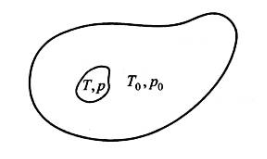
\includegraphics[width=6cm]{Ther_smallsystem.png}
		\caption{一个包含子系统的孤立均匀系统}
		\label{figure_1}
	\end{wrapfigure}

	考虑一个孤立的均匀系统中的任意一个小部分,这部分虽小,但仍含有大量的微观粒子,可以看做一个宏观系统。(见图\ref{figure_1})将这小部分成为子系统,而把系统的其他部分看做子系统的介质。将不带下标的量表示子系统的热力学量,下标0的表示介质的热力学量。


	设想子系统发生一个虚变动,造成了内能和体积的变化,由于整个系统是孤立的,可以得到
	\begin{equation}
	\begin{array}{l}{\delta U+\delta U_{0}=0} \\ {\delta V+\delta V_{0}=0}\end{array}
	\end{equation}
	
\noindent 熵是广延量,虚变动导致整个系统的熵变为$ \Delta \tilde{S} = \Delta S + \Delta S_{0} $,将$ S $和$ S_{0} $作泰勒展开,准确到二级,得到
\begin{equation}
\begin{aligned} \Delta S &=\delta S+\frac{1}{2} \delta^{2} S \\ \Delta S_{0} &=\delta S_{0}+\frac{1}{2} \delta^{2} S_{0} \end{aligned}
\end{equation}

\noindent 在稳定的平衡条件下,整个孤立系统的熵应取最大值,熵函数的极值要求
\begin{equation}
\delta \tilde{S}=\delta S+\delta S_{0}=0
\end{equation}

\noindent 考虑热力学基本方程可以得到
\begin{equation}
\delta \tilde{S}=\delta U\left(\frac{1}{T}-\frac{1}{T_{0}}\right)+\delta V\left(\frac{p}{T}-\frac{p_{0}}{T_{0}}\right)=0
\end{equation}

\noindent 由于在虚变动中$ \delta U $和$ \delta V $可以独立地改变,所以$ \tilde{S} = 0 $要求
\begin{equation}
T=T_{0}, \quad p=p_{0}
\end{equation}

\noindent 由此知道平衡条件为子系统与介质具有相同的温度和压强,考虑到在图\ref{figure_1}中选取的子系统具有任意性,这意味着达成平衡时整个系统的温度和压强是均匀的。


	如果熵函数的二级微分是负的,即
	\begin{equation}
	\delta^{2} \tilde{S}=\delta^{2} S+\delta^{2} S_{0}<0\label{equ_S}
	\end{equation}
	
\noindent 则熵函数将具有极大值。由于介质比子系统大得多,可以忽略介质的熵的变化\footnote{通过考虑熵的广延量和一阶偏导的强度量性质得到二阶偏导量和物质的量的关系可以知道为何能够忽略介质的熵的变化},因此可以将\ref{equ_S}近似为
\begin{equation}
\delta^{2} \tilde{S} \approx \delta^{2} S<0
\end{equation}

	根据泰勒展开公式,得到
	\begin{equation}
	\delta^{2} S=\left[\left(\frac{\partial^{2} S}{\partial U^{2}}\right)(\delta U)^{2}+2 \frac{\partial^{2} S}{\partial U \partial V} \delta U \delta V+\left(\frac{\partial^{2} S}{\partial V^{2}}\right)(\delta V)^{2}\right]<0
	\end{equation}
	
\noindent 选$ T,V $为独立变量,通过导数变化可以得到(具体证明过程见书本)
\begin{equation}
\delta^{2} S=-\frac{C_{v}}{T^{2}}(\delta T)^{2}+\frac{1}{T}\left(\frac{\partial p}{\partial V}\right)_{T}(\delta V)^{2}<0
\end{equation}

\noindent 如果要求$ \delta^{2} S $对各种可能的虚变动都为负值,则要求
\begin{equation}
C_{V}>0, \quad\left(\frac{\partial p}{\partial V}\right)_{T}<0
\end{equation}

\noindent 这便是平衡的稳定条件。如果子系统对平衡发生某种偏离,系统中将会自发产生上述相应过程,以恢复系统的平衡。

	\subsection{开系的热力学基本方程}
	考虑单元系的相变时需要考虑开系,即一个系的质量或物质的量是可以改变的,具体到相变中即是某一个相的质量或物质的量可以改变。
	
	对于开系,从吉布斯函数开始考虑,增加一个反映物质的量发生变化的量
	\begin{equation}
	\mathrm{d} G=-\operatorname{Sd} T+V \mathrm{d} p+\mu \mathrm{d} n
	\end{equation}
	
\noindent 其中
\begin{equation}
\mu=\left(\frac{\partial G}{\partial n}\right)_{T, p}
\end{equation}

\noindent 便被称为化学势。考虑到吉布斯函数的广延量性质,
\begin{equation}
G(T, p, n)=n G_{m}(T, p)
\end{equation}

\noindent 因此
\begin{equation}
\boldsymbol{\mu}=\left(\frac{\partial G}{\partial n}\right)_{T,p}=G_{m}
\end{equation}

\noindent 这表明,化学势等于摩尔吉布斯函数,这个结果仅适用于单元系。

	开系的热力学基本方程为
	\begin{equation}
	\mathrm{d} U=T \mathrm{d} S-p \mathrm{d} V+\mu \mathrm{d} n
	\end{equation}
	
\noindent 容易推得焓和自由能的全微分方程。在此基础之上引入一个新的热力学函数
\begin{equation}
J=F-\mu n
\end{equation}

\noindent 称为\textbf{巨热力势},它的全微分为
\begin{equation}
\mathrm{d} J=-S \mathrm{d} T-p \mathrm{d} V-n \mathrm{d} \mu
\end{equation}

\noindent 在近独立粒子和巨正则系综部分它还会出场。

	\subsection{单元系的复相平衡条件}
	考虑一个单元二相系,整体作为一个孤立系统。由于整个系统是孤立系统,它的总内能、总体积和总物质的量应该是恒定的。应用虚功原理,由于孤立系条件,在虚变动中总的内能、体积和物质的量的变化应该为0。
	
	考虑熵的广延量性质,整个系统的熵变为
	\begin{equation}
	\delta S=\delta S^{\alpha}+\delta S^{\beta}=\delta U^{a}\left(\frac{1}{T^{a}}-\frac{1}{T^{\beta}}\right)+\delta V^{a}\left(\frac{p^{\alpha}}{T^{\alpha}}-\frac{p^{\beta}}{T^{\beta}}\right)-\delta n^{\alpha}\left(\frac{\mu^{\alpha}}{T^{\alpha}}-\frac{\mu^{\beta}}{T^{\beta}}\right)
	\end{equation}
	
\noindent 同样考虑平衡条件$ \delta S = 0 $,且考虑到$ \delta U^{\alpha}, \delta V^{\alpha}, \delta n^{\alpha} $ 三者是独立改变的,可得
\begin{equation}
	\begin{aligned}
	\frac{1}{T^{a}}-\frac{1}{T^{\beta}}&=0
	\\
	\frac{p^{ \alpha}}{T^{a}}-\frac{p^{\beta}}{T^{\beta}}=0
	\\
	\frac{\mu^{\alpha}}{T^{\alpha}}-\frac{\mu^{\beta}}{T^{\beta}}=0
	\end{aligned}
\end{equation}

\noindent 即
\begin{equation}
\begin{array}{l}{T^{\alpha}=T^{\beta}} \\ {p^{\alpha}=p^{\beta}} \\ {\mu^{\alpha}=\mu^{\beta}}\end{array}
\end{equation}

\noindent 分别对应热平衡条件、力学平衡条件和相变平衡条件。

	如果平衡条件未能满足,复相系将发生变化,变化是朝着熵增加的方向进行的。由此可以很快推知在不同的不平衡条件下,系统会发生怎样的变化以达到平衡条件。
	
	\subsection{单元复相系的平衡性质}
	考虑单元系相图
	\begin{figure}[ht]
		\centering
		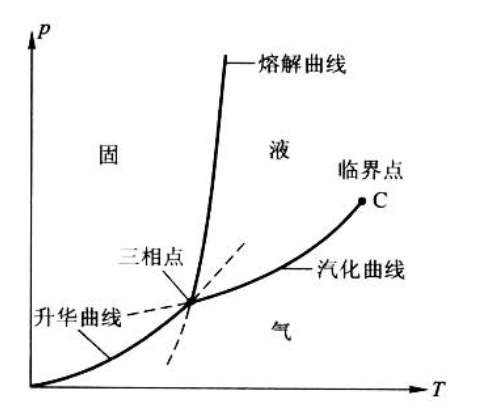
\includegraphics[width=12cm]{Ther_equilibrium.png}
		\caption{单元系相图}
		\label{figure_2}
	\end{figure}

\noindent 由图\ref{figure_2}可以看出,三条曲线正好将图分成三个区域,分别是固相、液相和气相单相存在的温度和压强范围。三条曲线分别为升华线、熔解线和汽化线,在曲线上可以实现对应相的两相平衡共存。在三相点处三相可以共存。汽化线上有一临界点,温度高过此点将不存在液体。

	两相的转变可以视作相图上穿过三条曲线的运动。在与曲线相交时放出热量,称为\textbf{相变潜热},此时温度和压强保持不变 ,不同的相的物质的量发生变化。当相变过程结束后,运动继续,直到终点。
	
	相图的结构可以通过热力学理论予以解释。由于化学势是压强和温度函数,则在一定的压强和温度范围下,系统的平衡位置即是化学势最小的状态,如果某一相$ \alpha $的化学势较其他相低,这个范围即是$ \alpha $相的单相区域。
	
	在平衡曲线上满足复相系的三条平衡条件,此时温度和压强两个参量只有一个可以独立改变,两相可以以任意比例共存,整个系统的吉布斯函数都是相等的。
	
	根据热力学理论可以求出两相平衡曲线的斜率。考虑曲线上相邻的两点,在这两点上,两相的化学势都相等:
	\begin{equation}
	\begin{aligned} \mu^{a}(T, p) &=\mu^{\beta}(T, p) \\ \mu^{\alpha}(T+\mathrm{d} T, p+\mathrm{d} p) &=\mu^{\beta}(T+\mathrm{d} T, p+\mathrm{d} p) \end{aligned}
	\end{equation}
	
\noindent 两式相减可得
\begin{equation}
\mathrm{d} \mu^{\alpha}=\mathrm{d} \mu^{\beta}
\end{equation}

\noindent 考虑化学势的全微分$\mathrm{d} \mu=-S_{m} \mathrm{d} T+V_{m} \mathrm{d} p$,可以得到
\begin{equation}
\frac{\mathrm{d} p}{\mathrm{d} T}=\frac{S_{m}^{\beta}-S_{m}^{\alpha}}{V_{m}^{\beta}-V_{m}^{\alpha}}
\end{equation}

\noindent 其中下标m表示为单摩尔对应的量。以$ L $表示1 mol 物质$ \alpha \rightarrow \beta $时所吸收的相变潜热,考虑到相变时温度不变,故
\begin{equation}
L=T\left(S_{m}^{\beta}-S_{m}^{\alpha}\right)
\end{equation}

\noindent 由此得到
\begin{equation}
\frac{\mathrm{d} p}{\mathrm{d} T}=\frac{L}{T\left(V_{m}^{\mathrm{\beta}}-V_{m}^{\alpha}\right)}
\end{equation}

\noindent 该式被称为\textbf{克拉珀龙方程},它给出了两相平衡曲线的斜率。

	由克拉珀龙方程可以推导蒸气压方程。与凝聚相(液相或固相)达到平衡的蒸汽称为\textbf{饱和蒸汽}。
	
	以$ \alpha $相表示凝聚相,$ \beta $相表示气相,考虑到凝聚相的摩尔体积远小于气相的摩尔体积,则可略去$ V_{m}^{\alpha} $,并把气相看作理想气体$p V_{m}^{\beta}=R T$,可以得到
	\begin{equation}
	\frac{1}{p} \frac{\mathrm{d} p}{\mathrm{d} T}=\frac{L}{R T^{2}}
	\end{equation}
	
\noindent 如果粗糙地认为相变潜热与温度无关,可以积分得到
\begin{equation}
\ln p=-\frac{L}{R T}+A
\end{equation}

\noindent 这便是蒸气压方程的近似表达式。

	\subsection{临界点和气液两相的转变}
	\subsubsection{以二氧化碳为例分析气液转变的特性}
	\begin{figure}[ht]
		\begin{minipage}[t]{0.5 \linewidth}
			\centering
			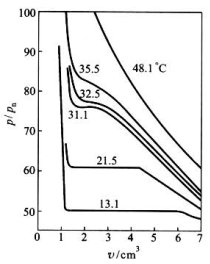
\includegraphics[width=6cm]{Ther_CO2.png}
			\caption{高温下二氧化碳的等温线}
			\label{figure_3}
		\end{minipage}
		\begin{minipage}[t]{0.5 \linewidth}
			\centering
			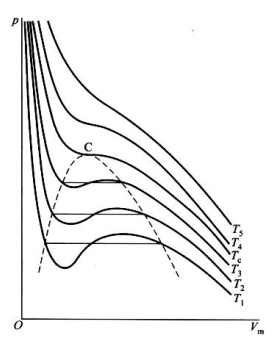
\includegraphics[width=6cm]{Ther_fangde.png}
			\caption{范氏气体等温线图}
			\label{figure_4}
		\end{minipage}
	\end{figure}

	通过二氧化碳在高温下的等温线图可以得知,在临界温度之上,等温线的形状与玻意耳定律给出的双曲线近似,是气相的等温线。在临界温度一下,等温线包括三段:左边的几乎与$ p $轴平行,代表液相;右边的一段代表气相,而中间的和$ v $轴平行的直线代表气液共存。
	
	对于单位质量的物质,这段直线的左端的横坐标是液相的比体积$ v_{1} $,右端的横坐标是气相的比体积$ v_{2} $,直线中体积为$ v $的一点,相应的液相比例$ x $和气相比例$ 1-x $由下式给出
	\begin{equation}
	v=x v_{1}+(1-x) v_{g}
	\end{equation}
	
	等温线中的水平段随温度的升高而缩短,当温度处于某一极限温度时,水平段的左右端重合,这时两相的比体积相等,物质处于液、气部分的状态。这一极限温度就是临界温度$ T_{C} $,相应的压强是临界压强$ p_{C} $.
	
	考虑范德瓦尔斯方程,对于1mol物质,
	\begin{equation}
	\left(p+\frac{a}{V_{m}^{2}}\right)\left(V_{m}-b\right)=R T
	\end{equation}
	

	比较图\ref{figure_3}和图\ref{figure_4}可以发现有一些状态由于不满足平衡稳定性条件的要求因而不能作为均匀系而实现。现在通过吉布斯函数最小的要求,讨论什么状态才是稳定的状态。
	
	化学势的全微分是
	\begin{equation}
	\mathrm{d} \mu=-S_{m} \mathrm{d} T+V_{\mathrm{m}} \mathrm{d} p
	\end{equation}
	
\noindent 容易得到,等温线上不同压强之间的化学势之差为
\begin{equation}
\mu-\mu_{0}=\int_{p_{0}}^{p} V_{m} \mathrm{d} p
\end{equation}

	\begin{wrapfigure}{r}{6cm}
		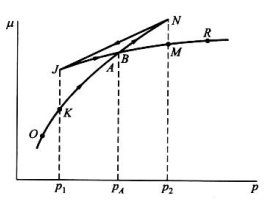
\includegraphics[width=6cm]{Ther_huaxueshi.png}
		\caption{等温线上的化学势变化情况}
		\label{figure_5}
	\end{wrapfigure}

	化学势在等温线上随压强的变化见图\ref{figure_5},图中出现一个$ p $值对应多个$ \mu $的情况,根据吉布斯函数判据,可以得知代表系统呢稳定平衡状态的是线段OKBAMR.
	
	在B点物质全部处在气态,在A点物质全部处在液态,两点的$ \mu $值相等,这正是相变平衡条件。这个条件相当于
	\begin{equation}
	\int_{B N D J A} V_{\mathrm{m}} \mathrm{d} p=0
	\end{equation}
	
\noindent 这称为麦克斯韦等面积法则。根据等面积法则,可以将范氏气体等温线中的BNDJA段换为直线BA.

	在线段JND上的状态不满足平衡稳定性的要求,物质不可能作为均匀系存在而必将发生相变;线段BN和AJ的状态满足平衡稳定性的要求,由于其化学势高于两相平衡的化学势,它们可以作为亚稳态单相存在,分别对应于\textbf{过饱和蒸汽}和\textbf{过热液体}。
	
	\subsubsection{液气流体系统临界态的平衡稳定条件}
	现在根据热力学的一般论据证明,液气流体系统临界态的平衡稳定条件(与物态方程的具体表达式无关)为
	\begin{equation}
	\left(\frac{\partial p}{\partial V_{m}}\right)_{T}=0, \left(\frac{\partial^{2} p}{\partial V_{m}^{2}}\right)_{T}=0,\left(\frac{\partial^{3} p}{\partial V_{m}^{3}}\right)_{T}<0
	\end{equation}
	
\noindent 如前所述,液气两相平衡时,两相具有相同的温度和压强。在接近临界点的等温线上,两相平衡时其摩尔体积是接近的。以$ V_{m} $和$ V+\delta V_{m} $分别表示液相和气相的摩尔体积,两相压强相等可以表达为
\begin{equation}
p\left(V_{m}, T\right)=p\left(V_{m}+\delta V_{m}, T\right)\label{equ_p}
\end{equation}

\noindent 根据一般套路,即进行泰勒展开,并准确到第二级,可得
\begin{equation}
p\left(V_{m}+\delta V_{m}, T\right)=p\left(V_{m}, T\right)+\left(\frac{\partial p}{\partial V_{m}}\right)_{T} \delta V_{m}+\frac{1}{2}\left(\frac{\partial^{2} p}{\partial V_{m}^{2}}\right)_{T}\left(\delta V_{m}\right)^{2}
\end{equation}

\noindent 代入式\ref{equ_p},全式除以$ \delta V_{m} $,可得

\begin{equation}
\left(\frac{\partial p}{\partial V_{m}}\right)_{T}+\frac{\delta V_{m}}{2}\left(\frac{\partial^{2} p}{\partial V_{m}^{2}}\right)_{T}=0
\end{equation}

\noindent 当$ T \rightarrow T_{C} $时,$ \delta V_{m} $趋于零,由此可知在临界点有
\begin{equation}
\left(\frac{\partial p}{\partial V_{m}}\right)_{T}=0
\end{equation}

\noindent 上式指出,处在临界点的液气流体系统不满足平衡稳定条件的第二式,这是临界态的特性决定的。如果将系统约束在临界温度上,可以得到$ \delta^{2} S_{m}=0 $

	为了分析液气流体系统临界态的平衡稳定性,将$ \Delta S_{m} $的展开扩展为
	\begin{equation}
	\Delta S_{m}=\delta S_{m}+\frac{1}{2 !} \delta^{2} S_{m}+\frac{1}{3 !} \delta^{3} S_{m}+\frac{1}{4 !} \delta^{4} S_{m}+\cdots
	\end{equation}
	
\noindent 根据之前的结果
\begin{equation}
\delta^{2} S_{m}=-\frac{C_{V, m}}{T^{2}}(\delta T)^{2}+\frac{1}{T}\left(\frac{\partial p}{\partial V_{m}}\right)_{T}\left(\delta V_{m}\right)^{2}
\end{equation}

\noindent 同时考虑到
\begin{equation}
\delta^{3} S_{m}=\left(\frac{\partial}{\partial T} \delta^{2} S_{m}\right) \delta T+\left(\frac{\partial}{\partial V_{m}} \delta^{2} S_{m}\right) \delta V_{m}
\end{equation}

\noindent 可知,将系统约束在临界温度$ T_{C} $的情况下
\begin{equation}
\delta^{3} S_{m}=\frac{1}{T}\left(\frac{\partial^{2} p}{\partial V_{m}^{2}}\right)_{T}\left(\delta V_{m}\right)^{3}
\end{equation}

\noindent 考虑到系统的平衡稳定性不应该取决于虚变动中体积的变化,因而得到
\begin{equation}
\left(\frac{\partial^{2} p}{\partial V_{m}^{2}}\right)_{T}=0
\end{equation}

\noindent 最后考虑$ \delta^{4} S_{m} $,类似约束在临界温度下可以得到
\begin{equation}
\delta^{4} S_{m}=\frac{1}{T}\left(\frac{\partial^{3} p}{\partial V_{m}^{3}}\right)_{T}\left(\delta V_{m}\right)^{4}
\end{equation}

\noindent 平衡稳定性要求$\delta^{4} S_{m}<0$,因此
\begin{equation}
\left(\frac{\partial^{3} p}{\partial V_{m}^{3}}\right)_{T}<0
\end{equation}

	\subsection{液滴的形成}
	\subsubsection{液滴表面的压强关系}
	本部分以液滴的形成为例,讨论表面相对相变的影响。
	
	设液滴为$ \alpha $相,蒸气为$ \beta $相,表面为$ \gamma $相。将表面理想化为集合面,因此可以忽略表面相的物质的量。三相的热力学基本方程如下
	\begin{equation}
	\begin{array}{l}{\mathrm{d} U^{\alpha}=T^{\alpha} \mathrm{d} S^{\alpha}-p^{\alpha} \mathrm{d} V^{\alpha}+\mu^{\alpha} \mathrm{d} n^{\alpha}} \\ {\mathrm{d} U^{\beta}=T^{\beta} \mathrm{d} S^{\beta}-p^{\beta} \mathrm{d} V^{\beta}+\mu^{\beta} \mathrm{d} n^{\beta}} \\ {\mathrm{d} U^{\gamma}=T^{\gamma} \mathrm{d} S^{\gamma}+\sigma \mathrm{d} A}\end{array}
	\end{equation}
	
\noindent 假定热平衡条件已经满足,使用自由能判据推求系统的力学平衡条件和相变平衡条件。老套路了,使用虚功原理,注意是在温度和总体积不变的条件下发生一个虚变动,在这过程中总物质的量和总体积保持不变,而三相自由能的变化分别为
	\begin{equation}
	\begin{aligned} \delta F^{\alpha} &=-p^{\alpha} \delta V^{\alpha}+\mu^{\alpha} \delta n^{\alpha} \\ \delta F^{\beta} &=-p^{\beta} \delta V^{\beta}+\mu^{\beta} \delta n^{\beta} \\ \delta F^{\gamma} &=\sigma \delta A \end{aligned}
	\end{equation}
	
\noindent 在三相温度相等的情况下,整个系统的自由能是三相的自由能之和\footnote{通过$ F = U - TS $可以得到}。假设液体是球形的,半径为$ r $,可以得到
	\begin{equation}
	V^{a}=\frac{4 \pi}{3} r^{3}, A=4 \pi r^{2}
	\end{equation}
	
\noindent 于是可以得到总的自由能变化为
\begin{equation}
\delta F=-\left(p^{a}-p^{\beta}-\frac{2 \sigma}{r}\right) \delta V^{\alpha}+\left(\mu^{a}-\mu^{\beta}\right) \delta n^{a}
\end{equation}

\noindent 根据自由能判据得到
\begin{equation}
\begin{array}{c}{p^{\alpha}=p^{\beta}+\frac{2 \sigma}{r}} \\ {\mu^{\alpha}=\mu^{\beta}}\end{array}
\end{equation}

\noindent 这便是加入表面相的力学平衡条件和相变平衡条件。力学平衡条件指出,由于表面张力有使液滴收缩的趋势,液滴的压强必须大于蒸汽的压强才能维持力学平衡。

	现在来讨论液滴的形成问题。由于液滴的表面为曲面,参考液面为平面的情况,设气液两相平衡时蒸气的压强为$ p^{\prime} $,根据相变平衡条件可得
	\begin{equation}
	\mu^{\alpha}\left(p^{\prime}+\frac{2 \sigma}{r}, T\right)=\mu^{\beta}\left(p^{\prime}, T\right)
	\end{equation}
	
	由于当压强改变时,液体的性质改变很小,可以将液滴的化学势按压强展开,只取线性项,得到
	\begin{equation}
	\begin{aligned} \mu^{\alpha}\left(p^{\prime}+\frac{2 \sigma}{r}, T\right) &=\mu^{\alpha}(p, T)+\left(p^{\prime}-p+\frac{2 \sigma}{r}\right) \frac{\partial \mu^{\alpha}}{\partial p} \\ &=\mu^{\alpha}(p, T)+\left(p^{\prime}-p+\frac{2 \sigma}{r}\right) v^{\alpha} \end{aligned}
	\end{equation}
	
\noindent 这时再考虑蒸气的化学势。将其视为理想气体,根据理想气体的吉布斯函数\footnote{这个推导过程见第二部分,有些繁复,但结论挺重要}$ G_{m} = RT (\varphi + \ln p) $可得
\begin{equation}
\mu^{\beta}\left(p^{\prime}, T\right)=\mu^{\beta}(p, T)+R T \ln \frac{p^{\prime}}{p}
\end{equation}

\noindent 所以得到
\begin{equation}
\left(p^{\prime}-p+\frac{2 \sigma}{r}\right) v^{\alpha}=R T \ln \frac{p^{\prime}}{p}
\end{equation}

	考虑到实际中通常有$ p^{\prime} - p \ll \frac{2 \sigma}{r} $,上式可近似为
	\begin{equation}
	\ln \frac{p^{\prime}}{p}=\frac{2 \sigma v^{a}}{R T r}
	\end{equation}
	
	\subsubsection{过饱和蒸气的形成}
	在一定的温度和蒸气压强$ p^{\prime} $下,,与蒸气达到平衡的液滴半径$ r_{c} $为
	\begin{equation}
	r_{\mathrm{c}}=\frac{2 \sigma v^{\alpha}}{R T \ln \frac{p^{\prime}}{p}}
	\end{equation}
	
\noindent 这被称为\textbf{中肯半径},是液滴将继续凝结和汽化消失的分界线。

	在蒸气中液体的凝结是通过先形成微小液滴然后逐渐生长的方式发生的,如果在蒸气中不存在凝结核(例如灰尘或带电微粒等),由涨落而形成的液滴往往过小,不能增大,因此在非常干净的蒸气中,蒸气的压强可以超过饱和蒸气压而不凝结,形成过饱和蒸气。
	
	\subsubsection{过热液体的形成}
	对于液体中的气泡可以作同样的考虑。如果仍然令$ \alpha $相表示液相而$ \beta $相表示气相,则进行对$ r \rightarrow  -r $的变换之中可以得到
	\begin{equation}
	p^{\beta}=p^{a}+\frac{2 \sigma}{r}
	\end{equation}
	
\noindent 上式指出,气泡内蒸气的压强必须大于液体的压强才能维持力学平衡,同理可以得到
\begin{equation}
\ln \frac{p}{p^{\prime}}=\frac{2 \sigma v^{\alpha}}{R T r}
\end{equation}

\noindent 所以为满足相变平衡条件,气泡内的压强必须小于同温度的饱和蒸气压。

	基于此可以解释液体沸腾前的过热现象。液体沸腾时,液体内部有大量的气泡形成,使气液分界面大大增加,于是整个液体剧烈汽化。一般情况下,液体中溶有空气,这些既有的空气泡作核形成的气泡具有足够大的半径,分界面接近为平面,使得只要气泡中的蒸气压等于液体的压强时即能发生沸腾。
	
	但如果没有现存的气泡作核,依靠涨落形成的气泡半径很小,当达到正常沸点的温度时,力学平衡要求气泡内蒸气压强大,相变平衡条件又提出了相反的要求,这是没法同时满足的,除非液体的温度高于正常的沸点,使得相应的饱和蒸气压大于液体的压强,这便是形成过热液体的原因。
	
	\subsection{相变的分类}
	目前人类习惯上只把相变区分为一级相变和连续相变,即把原来的二级、三级等等相变统称为连续相变。
	
	一级相变意味着在相变点两相的化学势连续但一级偏导数存在突变,连续相变则是一级偏导数连续而高级的偏导数发生突变。由此会得到相变潜热、比体积、定压比热等物理量的不同性质。
	
	考虑二级相变在邻近的相变点的比熵和比体积变化相等,可以得到二级相变点压强随温度变化的斜率公式,即
	\begin{equation}
	\begin{aligned}\frac{\dif p}{\dif T}&=\frac{\alpha^{(2)}-\alpha^{(1)}}{\kappa_{T}^{(2)}-\kappa_{r}^{(1)}} 
		\\ 
	\frac{\dif p}{\dif T}&=\frac{c_{p}^{(2)}-c_{p}^{(1)}}{T v\left(\alpha^{(2)}-\alpha^{(1)}\right)}\end{aligned}
	\end{equation}
	
\noindent 这被称为\textbf{爱伦费斯特方程}。

	\subsection{朗道连续相变理论}
	
	\begin{wrapfigure}{r}{6cm}
		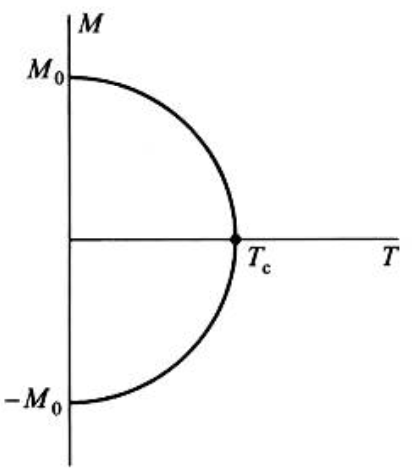
\includegraphics[width=6cm]{Ther_langdao.png}
		\caption{单轴各向异性铁磁体的序参量随温度的变化}
		\label{figure_6}
	\end{wrapfigure}

	朗道试图对连续相变提供一个统一的描述,他提出了序参量的概念,认为连续相变的特征是\textbf{物质有序程度的改变及与之相伴随的物质对称性质的变化}。
	
	考虑三维各向同性的铁磁体,将所有原子的磁矩取向都相同时认为是磁完全有序的状态,因而可以用自发磁化强度$ M(T) $作为序参量来描述铁磁物质的有序程度。

	单轴铁磁体具有一个容易磁化的晶轴,使得序参量的自由度为1,正值对应于磁矩向上。下面通过单轴铁磁体介绍朗道相变理论。
	
	朗道认为,在临界点$ T_{C} $附近,序参量$ M $是一个小量,可以将自由能在其附近进行展开,称为朗道自由能
	\begin{equation}
	F(T, M)=F_{0}(T)+\frac{1}{2} a(T) M^{2}+\frac{1}{4} b(T) M^{4}+\cdots
	\end{equation}
	
\noindent 由此系统变换对于$ M \rightarrow - M $是对称的,所以展开式不含奇次项。假设体积的变化可以忽略,并不失一般性地令其为单位提及,这样状态参量就只有温度了\footnote{注意,虽然写做$ F(T,M) $,但M并不是自变量}。
	
	稳定平衡态下自由能具有最小值,因此
	\begin{equation}
	\begin{aligned}\frac{\partial F}{\partial M}&=M\left(a+b M^{2}\right)=0 
	\\
	 \frac{\partial^{2} F}{\partial M^{2}}&=a+3 b M^{2}>0\end{aligned}
	\end{equation}
	
\noindent 由此得到三个解
\begin{equation}
M=0, M=\pm \sqrt{-\frac{a}{b}}
\end{equation}

\noindent 第一个解对应于$ T \geq T_{C} $的温度范围,表示无序态;后两个解则表示有序态。代入可知,在$ T<T_{C} $时,$ a<0 $.为了使序参量满足假设:在临界点处连续,可以得到$ a=0 $,,因此在临界点的领域可以简单地假设
\begin{equation}
a=a_{0}\left(\frac{T-T_{C}}{T_{C}}\right)=a_{0} t, a_{0}>0
\end{equation}

\noindent 以及$ b(T) = b = const $.

	在此基础上可以得到与临界点相关的一些物理量,结果感觉不是很重要,此处不再赘述。
	
	\section{多元系的复相平衡和化学平衡}\footnote{这一部分和下一部分由于时间有限,会较为简略}
	多元系时含有两种或两种以上化学组分的系统。多元系可以是均匀西,也可以是复相系。在多元系中既可以发生相变,也可以发生化学变化。
	
	\subsection{多元系的热力学函数和热力学方程}
	之后的讨论都设多元均匀系中含有$ k $个组元。由于可能发生相变或化学变化,均匀系中各组元物质的数量可能发生变化,需要引进各组元的质量或者物质的量作为描述平衡态的状态参量,即引进\textbf{化学参量}。
	
	这$ k $的化学参量并不是相互独立的,需要满足相变平衡条件或化学平衡条件,在以后的讨论中,将采取“先设为独立变量再引入约束”的方式处理。
	
	考虑$ T,p,n_{1},\cdots,n_{k} $为状态参量,可以得到系统的三个基本热力学函数体积、内能和熵
	\begin{equation}
	\begin{aligned} V &=V\left(T, p, n_{1}, \cdots, n_{k}\right) \\ U &=U\left(T, p, n_{1}, \cdots, n_{k}\right) \\ S &=S\left(T, p, n_{1}, \cdots, n_{k}\right) \end{aligned}
	\end{equation}
	
\noindent 根据体积、内能和熵的广延量性质可知,如果保持系统的温度和压强不变和令系统中各组元的物质的量都增为$ \lambda $倍,则系统的体积、内能和熵都增为$ \lambda $倍,这就是说,这三个函数时各组元物质的量的一次齐函数。

考虑齐次函数的\textbf{欧勒定理}:如果函数$f\left(x_{1}, \cdots, x_{k}\right)$满足如下条件
\begin{equation}
f\left(\lambda x_{1}, \cdots, \lambda x_{k}\right)=\lambda^{m} f\left(x_{1}, \cdots, x_{k}\right)
\end{equation}

\noindent 则这个函数称为对$ x_{1},\cdots, x_{k} $的$ m $次齐函数。对$ \lambda $求导再令其为1后可得
\begin{equation}
\sum_{i} x_{i} \frac{\partial f}{\partial x_{i}}=m f
\end{equation}

\noindent 这便是欧勒定理。

	由欧勒定理可得
	\begin{equation}
	\begin{aligned}V&=\sum_{i} n_{i}\left(\frac{\partial V}{\partial n_{i}}\right)_{T, p, n_{j}} \\ U&=\sum_{i} n_{i}\left(\frac{\partial U}{\partial n_{i}}\right)_{T, p, n_{j}} \\ S&=\sum_{i} n_{i}\left(\frac{\partial S}{\partial n_{i}}\right)_{T, p, n_{j}}\end{aligned}
	\end{equation}
	
\noindent 定义
\begin{equation}
v_{i}=\left(\frac{\partial V}{\partial n_{i}}\right)_{T, p, n_{j}}, \quad u_{i}=\left(\frac{\partial U}{\partial n_{i}}\right)_{T, p, n_{j}}, \quad s_{i}=\left(\frac{\partial S}{\partial n_{i}}\right)_{T, p, n_{j}}
\end{equation}

\noindent 可得更为简便的形式\footnote{注意上式偏导的下标j表示除i组元外的其他全部组元}
\begin{equation}
\begin{aligned}V=\sum_{i} n_{i} v_{i} \\ U=\sum_{i} n_{i} u_{i} \\ S=\sum_{i} n_{i} s_{i}\end{aligned}
\end{equation}

	显然,任何广延量都是各组元物质的量的一次齐函数。对于吉布斯函数也可以写作
	\begin{equation}
	G=\sum_{i} n_{i}\left(\frac{\partial G}{\partial n_{i}}\right)_{T, p, n_{j}}=\sum_{i} n_{i} \mu_{i}\label{equ_G}
	\end{equation}
	
	考虑对式\ref{equ_G}求微分,并与吉布斯函数的全微分进行比较,可以得到
	\begin{equation}
	S \mathrm{d} T-V \mathrm{d} p+\sum n_{i} \mathrm{d} \mu_{i}=0\label{equ_GBS}
	\end{equation}

\noindent 上式被称为吉布斯关系,表明在$ k+2 $个强度量变数中,只有$ k+1 $个是独立的。

	焓、自由能和吉布斯函数在复相系中并不是时刻有定义的。对于焓来说,当且仅当各相的压强相同时,才有定义;对于自由能是各相的温度相等;对于吉布斯函数是各相的温度和压强都相等。定义方式均是广延量的定义,即系统的焓、自由能和吉布斯函数等于各相的代数和。
	
	\subsection{多元系的复相平衡条件}
	设两相$ \alpha $和$ \beta $都含有$ k $个组元,这些组元之间不发生化学反应,并设热平衡条件和力学平衡条件已经得到满足。考虑一个虚变动,在这虚变动中两相各组元的物质的量发生改变,在没有发生化学反应时为
	\begin{equation}
	\delta n_{i}^{a}+\delta n_{i}^{\beta}=0 \quad(i=1,2, \cdots, k)
	\end{equation}
	
\noindent 根据套路,考虑总的吉布斯函数的变化
\begin{equation}
\delta G=\delta G^{\alpha}+\delta G^{\beta}
\end{equation}

\noindent 得到
\begin{equation}
\delta G=\sum_{i}\left(\mu_{i}^{\alpha}-\mu_{i}^{\beta}\right) \delta n_{i}^{\alpha}
\end{equation}

\noindent 由吉布斯函数判据可得相变平衡条件
\begin{equation}
\mu_{i}^{\alpha}=\mu_{i}^{\beta} \qquad(i=1,2, \cdots, k)
\end{equation}

	留意一种平衡叫\textbf{膜平衡}。膜平衡使得只有能够流动的组元满足之前得出的力学平衡和相变平衡条件,对于其他物质则不必保持。
	
	\subsection{吉布斯相律}
	吉布斯相律考虑了多元复相系达到平衡时的独立参量数。
	
	设多元复相系有$ \varphi $个相,每个相有$ k $个组元,它们之间不发生化学反应。还和之前一样考虑温度、压强和各组元的物质的量作为每一个相的状态参量,同时考虑平衡条件。
	
	由于系统是否达到热动平衡条件是强度量决定的,总质量改变但这些强度量不变则系统的平衡没法被打破,所以为了确定相的强度量性质,考虑用各组元相对比例的强度量$ x_{i} $代替广延量$ n_{i} $作为状态参量。引入定义
	\begin{equation}
	x_{i}=\frac{n_{i}}{n}
	\end{equation}
	
	由于相对比例之和为1,所以$ k $个$ x_{i} $只有$ k-1 $个是独立的,加上温度和压强,描述一个相需要$ k+1 $个强度量变量,和吉布斯关系式\ref{equ_GBS}一致。但若要确定该相的广延量数值,还需要增加一个变量,即如该相的总物质的量,共$ k+2 $个变量\footnote{可以理解为从强度量到广延量的跨越需要引入针对系统整体大小进行描述的一个量}。
	
	再考虑要满足平衡条件,即
	\begin{equation}
	\begin{aligned}
	T^{1}&=T^{2}=\dots=T^{\varphi}
	\\
	P^{1}&=P^{2}=\dots=P^{\varphi}
	\\
	\mu^{1}_{i}&=\mu^{2}_{i}=\dots=\mu^{\varphi}_{i} \quad (i=1,2,\cdots,k)
	\end{aligned}
	\end{equation}
	
\noindent 这三个平衡条件共有$ (k+2)(\varphi-1) $个方程,因此得到独立改变的量为
\begin{equation}
f=(k+1) \varphi-(k+2)(\varphi-1) =k+2-\varphi
\end{equation}

\noindent 上式被称为吉布斯相律。

	在以上的证明中,做了每一个相都有$ k $个组元的假设,但如果该假设不成立,吉布斯相律的表达形式依旧成立,但这是$ k $个意义变为复相系中总的组元数,即
	\begin{equation}
		k=\max \{k_{1},k_{2},\cdots,k_{\varphi}\}
	\end{equation}
	
	\subsection{化学平衡条件}
	在可以发生化学反应时系统达到平衡所要满足的条件,称为化学平衡条件。简单起见,只讨论单相系下的化学反应,这种化学反应被称为单向化学反应。
	
	对于化学反应的表示,在热力学中写作如下模样
	\begin{equation}
	2 \mathrm{H}_{2} \mathrm{O}-2 \mathrm{H}_{2}-\mathrm{O}_{2}=0
	\end{equation}
	
\noindent 即直接用等式书写,不用可逆符号。方程中带有正系数的组元称为\textbf{生成物},带有负系数的组元称为\textbf{反应物}。由于实际上化学反应的方向与反应条件有关,因此反应方向和反应物、生成物的规定是带有任意性的。

	单向化学反应方程的一般形式为
	\begin{equation}
	\sum_{i} \nu_{i} A_{i}=0
	\end{equation}

\noindent 发生化学反应时,各组元物质的量的改变必须与各组元在反应方程中的系数成正比。

	令
	\begin{equation}
	\mathrm{d} n_{i}=\nu_{i} \mathrm{d} n(i=1,2, \cdots, k)
	\end{equation}
	
\noindent 则$ \dif n >0 $时反应正向进行,$ \dif n<0 $时反应逆向进行。
	
	以$ h_{i} $表示$ i $组元的偏摩尔焓,则在\textbf{等温等压条件下}发生化学反应以后得到系统焓的改变为
	\begin{equation}
	\Delta H=\sum_{i} \nu_{i} h_{i}
	\end{equation}
	
\noindent 考虑到在等压过程中焓的增加等于系统在过程中从外界吸收的热量,故
\begin{equation}
Q_{p}=\Delta H
\end{equation}

\noindent $ Q_{p} $称为化学反应的定压反应热。

	由于焓是态函数,可知$ \Delta H $的值与过程无关,这表明:如果一个反应可以通过不同的两组中间过程达到,两组过程的反应热应该相当。这个结果名为\textbf{赫斯定理}\footnote{就是那个在高考化学中承担了一个重要考点的定理}。
	
	现在讨论单向反应的平衡条件。假设反应是在等温等压条件下进行的,不用怀疑,还是使用老套路:虚功原理$ + $吉布斯函数判据,于是得到
	\begin{equation}
	\sum_{i} \nu_{i} \mu_{i}=0
	\end{equation}
	
\noindent 如果平衡条件未能满足,反应就要进行。反应进行的反向必然使得吉布斯函数减小,即
\begin{equation}
\delta n \sum_{i} \nu_{i} \mu_{i}<0
\end{equation}

\noindent 还可以写作$ \delta G = \delta H - T \delta S $,这便是高中判断化学反应方向的原理。

	如果给定初态下各组元的物质的量$ n_{1}^{0},\cdots,n_{k}^{0} $,终态各组元的物质的量将为
	\begin{equation}
	n_{i}=n_{i}^{0}+\nu_{i} \Delta n
	\end{equation}

\noindent 只要定出参量$ \Delta n $,就可以确定终态各组元的物质的量。

	现在考虑$ \Delta n $的取值。该值的取值应该使得任何$ n_{i} $都不应为负值。现在以$ \Delta n_{a} $表示其最大值,即反应正向进行的最大限度;令$ \Delta n_{b} $表示其最小值,即反应逆向进行的最小限度。由于$ \Delta n $的可能值处于两者之间,运用一个无比简单的高数技巧可以定义一个值域为$ [0,1] $的函数
	\begin{equation}
	\varepsilon=\frac{\Delta n-\Delta n_{b}}{\Delta n_{a}-\Delta n_{b}}
	\end{equation}
	
\noindent 该函数被称为反应度,当$ \varepsilon=1 $时表示正向反应达到最大限度;当$ \varepsilon=0 $时表示逆向反应达到最大限度。

	这里需要注意,通过化学平衡条件求得的$ \Delta  n $可能不在$ [\Delta n_{b}, \Delta n_{a}] $中,这意味着化学反应将由于某组元的耗尽而停止,这时系统并不满足化学平衡条件但反应已经完成。补充定义此时的反应度为1或0.
	
	\subsection{混合理想气体的性质}
	设混合气体含有$ k $个组元,各组元的物质的量分别为$ n_{1}, n_{2}, \cdots, n_{k} $.混合气体温度为$ T $,体积为$ V $.实验指出,混合气体的压强等于各组元的分压之和:
	\begin{equation}
	p=\sum_{i} p_{i}
	\end{equation}
	
\noindent 这被称为\textbf{道尔顿分压定律},只是低温下的极限形式,因而只适用于混合理想气体。

	由此并根据理想气体的物质方程可以得到混合理想气体的物态方式
	\begin{equation}
	p V=\left(n_{1}+n_{2}+\cdots+n_{k}\right) R T
	\end{equation}
	
\noindent 由此可以得到$ i $组元的分压与混合气体的总压强的关系
\begin{equation}
\frac{p_{i}}{p}=\frac{n_{i}}{n_{1}+\cdots+n_{k}}=x_{i}
\end{equation}

	可以根据一个有关半透膜的实验事实\footnote{一个能够通过半透膜的组元,它在膜两边的分压在平衡时相等}推求混合气体的内能和熵。假设半透膜一边是混合气体,另一边是纯$ i $组分气体,则达到平衡时,对于$ i $组分需要满足三条平衡方程,则可以根据纯理想气体的化学势求得
	\begin{equation}
	\mu_{i}=R T\left(\varphi_{i}+\ln p_{i}\right)=R T\left[\varphi_{i}+\ln \left(x_{i} p\right)\right]\label{equ_mu}
	\end{equation}
	
\noindent 其中
\begin{equation}
\varphi_{i}=\frac{h_{i 0}}{R T}-\int \frac{\mathrm{d} T}{R T^{2}} \int c_{p i} \mathrm{d} T-\frac{s_{i 0}}{R}
\end{equation}

\noindent 如果理想气体的热容量可以视为常量,则得到
\begin{equation}
\varphi_{i}=\frac{h_{i 0}}{R T}-\frac{c_{p i}}{R} \ln T+\frac{c_{p i}-s_{i 0}}{R}
\end{equation}

	根据式\ref{equ_G}可以得到混合理想气体的吉布斯函数为
	\begin{equation}
	G=\sum_{i} n_{i} \mu_{i}=\sum_{i} n_{i} R T\left[\varphi_{i}+\ln \left(x_{i} p\right)\right]
	\end{equation}
	
\noindent 由于之前推理吉布斯函数时将混合理想气体不同组分之间的联系都放在化学势上了,如今利用半透膜的模型便可以方便地得到混合理想气体中每一种组元的化学势情况了。

	得到吉布斯函数后便可以轻松地得到其他热力学函数了,如体积
	\begin{equation}
	V=\frac{\partial G}{\partial p}=\frac{\sum_{i} n_{i} R T}{p}
	\end{equation}
	
\noindent 可以发现和直接利用道尔顿分压定律得到的体积表达式一致,这从一个侧面说明之前用半透膜求得吉布斯函数的方式是合理的。还可以得到熵,由
\begin{equation}
S=-\frac{\partial G}{\partial T}
\end{equation}

\noindent 得到
\begin{equation}
S=\sum_{i} n_{i}\left[\int c_{p i} \frac{\mathrm{d} T}{T}-R \ln \left(x_{i} p\right)+s_{i0}\right]
\end{equation}

	其他诸如焓、内能都很容易可以推出,而且可以发现,它们都是各组元的分焓、分内能之和。从微观角度分析原因可认为是理想气体分子之间没有相互作用。
	
	再次考虑混合理想气体的熵,先改写成如下形式
	\begin{equation}
	S=\sum_{i} n_{i}\left[\int c_{p i} \frac{\mathrm{d} T}{T}-R \ln p+s_{i 0}\right]+C
	\end{equation}
	
\noindent 其中
\begin{equation}
C=-R \sum_{i} n_{i} \ln x_{i}
\end{equation}

\noindent 可知$ C > 0 $恒成立,而$ C $代表各组元气体在等温等压混合后的熵的变化,这说明这个过程是熵增过程,因而是不可逆的。

	在这基础上,可以知道对于两个具有同样物质的量的气体,在等温等压下进行混合,熵增为
	\begin{equation}
	C=2 n R \ln 2
	\end{equation}
	
\noindent 与气体的具体性质无关。在由性质任意接近的两种气体过渡到同种气体时,$ C $将突变为零,这被称为\textbf{吉布斯佯谬},是经典统计物理不能解释的。

	\subsection{理想气体的化学平衡}
	考虑化学反应的平衡条件
	\begin{equation}
	\sum_{i} \nu_{i} \mu_{i}=0
	\end{equation}
	
\noindent 将\ref{equ_mu}得到的化学势代入上式可得
\begin{equation}
R T \sum_{i} \nu_{i}\left[\varphi_{i}(T)+\ln p_{i}\right]=0
\end{equation}

\noindent 定义化学反应的定压平衡常量$ K_{p} $,简称为\textbf{平衡常量}
\begin{equation}
\ln K_{p}=-\sum_{i} \nu_{i} \varphi_{i}(T)
\end{equation}

\noindent 则可以将平衡条件表示为
\begin{equation}
\prod_{i} p_{i}^{\nu_{i}}=K_{p}(T)
\end{equation}

\noindent 上式给出了气体反应达到平衡时各组元分压之间的关系,成为\textbf{质量作用律}。进一步可得
\begin{equation}
\prod_{i} x_{i}^{\nu_{i}}=K(T, p)
\end{equation}

\noindent 其中$ K(T,p) $也被称为平衡常量。

	根据之前推得的结论,当化学反应平衡条件未被满足时,反应便要进行。根据之前的结论,反应正向进行的条件是
	\begin{equation}
	\sum_{i} \nu_{i} \mu_{i}<0
	\end{equation}
	
\noindent 所以
\begin{equation}
\prod_{i} p_{i}^{v_{i}}<K_{p}
\end{equation}

\noindent 所以如果知道平衡常量,则只要知道初始条件便可以知道达成平衡时各组元的物质的量。在这个基础之上可以出来一堆的计算题,希望梅老板不会做这么无聊的事情$ \cdots $

	\subsection{热力学第三定律}
	热力学第三定律有两种等价的表述,分别为\textbf{能氏定律}和\textbf{绝对零度不能达到原理},具体如下:
	
	能氏定律:凝聚系的熵在等温过程中的改变随绝对温度趋于零,即
	\begin{equation}
	\lim _{T \rightarrow 0}(\Delta S)_{T}=0
	\end{equation}
	
\noindent 其中$ (\Delta S)_{T} $指在等温过程中熵的改变。

	绝对零度不能到达定理:不可能通过\textbf{有限}的步骤使一个物体冷却到绝对温度的零度。
	
	能氏定理是在研究低温下熵变和焓变判据这两个不同的判据往往得出相似的结论的原因时提出的,作为一个假设引入从而解释在低温下两种判据的一致性的来源。能氏定理的正确性由之后的各种实验对其推论的证实而得到肯定。通过能氏定理可以得到温度趋于绝对零度时物质的一些形式:
	
	1、热容趋于零
	
	对于任意状态参量$ y $,在$ T \rightarrow 0 $时,可以得到
	\begin{equation}
	C_{y}=T\left(\frac{\partial S}{\partial T}\right)_{y}=\left(\frac{\partial S}{\partial \ln T}\right)_{y}
	\end{equation}
	
\noindent 由于熵有限,所以必然得到
\begin{equation}
\lim _{r \rightarrow 0} C_{y}=0
\end{equation}

	2、物质系统的熵与体积和压强无关,即
	\begin{equation}
	\lim _{T \rightarrow 0}\left(\frac{\partial S}{\partial p}\right)_{T}=0, \lim _{r \rightarrow 0}\left(\frac{\partial S}{\partial V}\right)_{p}=0
	\end{equation}
	
\noindent 由克拉珀龙方程
\begin{equation}
\frac{d p}{d T}=\frac{S_{2}-S_{1}}{V_{2}-V_{1}}
\end{equation}

\noindent 还可以推知,$ T \rightarrow 0 $时一级相变的 相平衡曲线为零。


	\section{不可逆过程热力学简介}
	\subsection{局域平衡 \enspace 熵流密度与局域熵产生率}
	
	对于一般系统的熵的变化可以作如下定义
	\begin{equation}
	\mathrm{d} S=\mathrm{d}_{e} S+\mathrm{d}_{\mathrm{i}} S
	\end{equation}
	
\noindent 其中$ \dif_{e} S $是由于系统与外界交换物质和能量所引起的系统熵变,是可正可负的;$ \dif_{i} S $表示系统内部发生的过程引起的熵产生,可逆为0,不可逆大于0.

	考虑热力学基本方程
	\begin{equation}
	T \mathrm{d} S=\mathrm{d} U+p \mathrm{d} V-\sum_{i} \mu_{i} \mathrm{d} N_{i}
	\end{equation}
	
\noindent 只讨论以下的情形:整个系统虽然处在非平衡状态,但如果将系统分成若干个小部分,由于各部分之间只通过界面区域的分子发生相互作用,且各小部分的弛豫时间比整个系统的弛豫时间要短得多,各个小部分就可以近似处在局域平衡的状态。由此可以直接使用在平衡条件下定义的各种物理量,对于广延量直接进行代数相加运算\footnote{实际处理中可能需要用到微积分}即可得到系统的对应量,对于强度量没有定义。

	略去基本方程的$ -p \dif V $\footnote{在不考虑流体力学问题的情况下},并将全式除以局域体积可以得到联系局域熵密度$ s $,内能密度$ u $和粒子数密度$ n_{i} $的方程式
	\begin{equation}
	T \mathrm{d} s=\mathrm{d} u-\sum_{i} \mu_{i} \mathrm{d} n
	\end{equation}
	
	在局域平衡情形下,可以将局域熵密度的增加率写成如下形式
	\begin{equation}
	\frac{\partial s}{\partial t}=-\nabla \cdot \boldsymbol{J}_{s}+\Theta
	\end{equation}
	
\noindent 式中$ \boldsymbol{J}_{s} $是单位时间内流过单位截面的熵,称为\textbf{熵流密度},$ \Theta $是单位时间内单位体积中产生的熵,称为\textbf{局域熵产生率}。整个系统熵的增加可以表示为
\begin{equation}
\begin{aligned} \frac{\mathrm{d} S}{\mathrm{d} t} &=\frac{\mathrm{d}}{\mathrm{d} t} \int s \mathrm{d} \tau=\int \frac{\partial s}{\partial t} \mathrm{d} \tau \\ &=\int\left[-\nabla \cdot J_{s}+\Theta\right] \mathrm{d} \tau \end{aligned}
\end{equation}

\noindent 利用高斯定理可得到
\begin{equation}
\frac{\mathrm{d} S}{\mathrm{d} t}=-\oint \boldsymbol{J}_{s} \cdot \mathrm{d} \boldsymbol{\sigma}+\int \Theta \mathrm{d} \tau
\end{equation}

\noindent 上式右方第一项表示单位时间内通过系统表面从外界流入的熵,第二项表示单位时间内系统各体积元的熵产生之和\footnote{这体现了熵增原理,即作为一个系统的熵是有净产生的}。比较可得
\begin{equation}
\frac{\mathrm{d}_{e} S}{\mathrm{d} t}=-\oint J_{s} \cdot \mathrm{d} \boldsymbol{\sigma}, \quad \frac{\mathrm{d}_{i} S}{\mathrm{d} t}=\int \Theta \mathrm{d} \tau
\end{equation}

\noindent 由于在任何宏观区域中熵产生都是正定的,故有$ \Theta \leq 0 $.
\end{document}